\chapter{Introdução}

O presente relatório discorre sobre um projeto que tem como objetivo auxiliar o condutor a realizar ultrapassagens em rodovias simples, de mão dupla, com segurança, a fim de evitar que motoristas tomem a decisão de fazer manobras arriscadas, baseados apenas na própria experiência ou bom senso.

Dentre os acidentes automotivos, os que possuem o maior número de vítimas fatais são do tipo colisão frontal. De 2010 a 2014 quase metade dos acidentes com fatalidades em rodovias federais, um total de 48,3\%, foram fruto desse tipo de colisão (24,6\%) e de atropelamentos (23,7\%). É um tipo de acidente que embora possua baixa ocorrência, representando apenas 4\% do total, é extremamente violento \cite{ipea}.

Essas informações recebem comprovação nos relatórios do IPEA, de 2008, informando que 81,75\% dos acidentes desse tipo ocorreram em pistas simples com tráfego nos dois sentidos e o principal motivo apontado seria: ultrapassagem indevida, ultrapassagem de veículos lentos ou em congestionamento e falta de visibilidade \cite{fatoresCondicionantesGravidade}.

Em outro relatório do IPEA, de 2004, mantém-se a mesma porcentagem apresentada no relatório recente de 2008 e que pode ser acompanhado na Figura 1 \cite{brasilTemMaisVitimasDeTransito}.

\begin{itemize}
	\item \textbf{Nome do projeto:} Sistema de Comunicação Interveicular para Alerta de Colisões em Rodovias (CIAC);

	\item \textbf{Descrição do Projeto:} Construção de um sistema que auxilie ultrapassagens com segurança em rodovias;

	\item \textbf{Gerentes do Projeto:} Tainara da Silva Costa e Renato Lucas Borges José de Carvalho.
\end{itemize}

\section{Tecnologia Existente}

\subsection{Sistema Toyota}

Apenas dois carros da marca Toyota foram contemplados com o novo sistema. São eles: RAV-4 hybrid e Lexus 2016 \cite{3comper}. No RAV4, o sistema anti colisão recebeu o nome de Toyota Safety Sense (TSS). O conjunto TSS permite o cliente pode optar pelo TSSC e TSSP. O primeiro também traz sistema de mudança de faixa e detector de farol alto. O segundo, destinado para veículos de médio e grande porte, oferece ainda Radar Cruise Control e detector de pedestres. No Lexus, a ferramenta é idêntica, porém recebeu um outro nome: Lexus Safety System + (LSS+).

O funcionamento desse sistema é apresentado em um vídeo disponibilizado pela Toyota. Nesse vídeo é possível perceber que o sistema foi criado para ser usado dentro e fora da cidade, trata-se um dispositivo que detecta possíveis casos de colisão. Tendo em vista a situação de perigo, um alerta é disparado para avisar ao condutor da provável colisão. Caso nenhuma iniciativa seja tomada para evitá-la, o próprio sistema aciona os freios e reduz a velocidade do veículo para 30km/h. O vídeo pode ser assistido pelo site: \cite{4comper}. O sistema é composto por uma câmera que trabalha em parceria com um radar e um laser. Entretanto, não é possível afirmar o modelo, a marca ou o exato funcionamento desses dispositivos. Entende-se, ao assistir o vídeo, que tanto os sensores quanto o radar estão localizados na parte frontal do veículo.

\begin{figure}[h!]
  \centering
  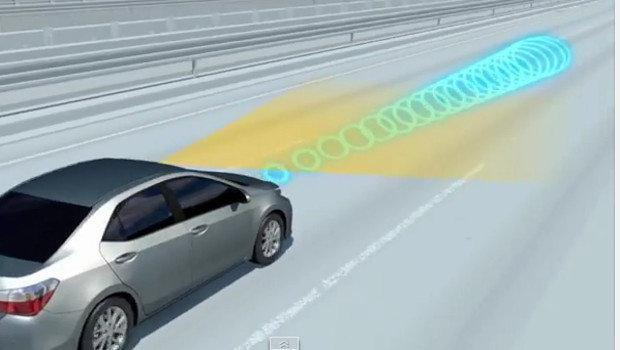
\includegraphics[width=350px, scale=0.5]{figuras/sinal_componentes}
  \caption{Revista Quatro Rodas}
\label{fig:sinal_componentes}
\end{figure}

\subsection{Sistema anticolisão VOLVO}

O Sistema de Alerta Anti Colisão com o Sistema de freio automático e o Sistema de detecção de ciclistas e pedestres é um recurso para axiliar os motoristas quando há risco de colisão com pedestres, ciclistas ou veículos na direção frontal que estão parados ou em movimento e de mesmo sentido do carro. 

\begin{figure}[h!]
  \centering
  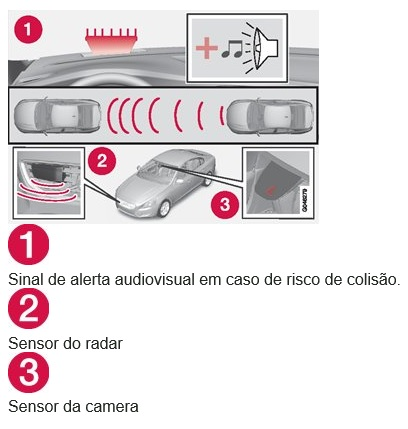
\includegraphics[width=350px, scale=0.5]{figuras/visao_geral}
  \caption{Visão Geral do sistema}
\label{fig:visao_geral}
\end{figure}

O Sistema não se aplica a todas as situações de condução ou de trânsito, condições de tempo ou de estrada. E ainda pode frear o carro ou diminuir a velocidade se houver risco de colisão, mas para assegurar o funcionamento é necessário que o motorista pressione o pedal do freio e também aconselha que o condutor nunca deve esperar pelo aviso de colisão, sempre seguir as leis de trânsito e manter uma distância segura do veículo da frente. 
O sistema anti colisão tem uma restrição sobre o alcance, ele só consegue detectar carros e objetos se estiverem em uma distância máxima de 150 metros \cite{volvo_system}. 

\section{Solução}

O sistema emitirá alertas de colisão indicando quando é seguro ultrapassar um veículo com o auxílio dos sensores LIDAR/RADAR, que possuem a função de detectar a distância de outros veículos; sensores de rotação e a câmera, que são capazes de identificar a intenção de ultrapassagem; um sistema de comunicação que utiliza a tecnologia dos transponders e dois módulos de GPS para auxiliar na identificação da posição do veículo. Este conjunto de equipamentos, juntamente com o microprocessador irão detectar os veículos ao redor, realizarão os cálculos em tempo real para determinar as distâncias e as velocidades, além da direção e do sentido dos mesmos, a fim de auxiliar o condutor na tomada de decisão da ultrapassagem ou alertá-lo caso esta não seja viável.

\section{Objetivo}

Espera-se que o projeto deste sistema seja capaz de auxiliar na construção e comercialização desta tecnologia de prevenção de acidentes e que todos os veículos contenham-na, a fim de que ela reduza os índices de colisões frontais nas rodovias brasileiras.

\section{Metodologia}

\subsection{Aplicação do Scrum ao CIAC}

Para o nosso processo de desenvolvimento, iremos utilizar o Scrum e como referência para este, o Guia do Scrum \cite{guiaScrum}.Nosso projeto adotará várias práticas desse modelo de gerenciamento, dentre elas a divisão interna dos times de desenvolvimento. Iremos dividir em três papeis chamados de Time Scrum: Product Owner, Time de Desenvolvimento e Scrum Master. 

Dentro de cada release, foram definidas várias sprints, cada uma com o timebox de uma semana. O marco para término da sprint é segunda feira, onde as atividades foram desenvolvidas até o dia anterior. Há um encontro presencial em todos os dias de término da sprint, onde, são executadas as reuniões de Revisão da Sprint, Retrospectiva da Sprint e Planejamento da Sprint contendo todas as equipes do projeto.

O projeto é composto por cinco times Scrum, cada um com seu Scrum master. O conjunto de Scrum masters é dirigido pelos dois Products Managers: Tainara Costa e Renato Carvalho. As demais equipes estão organizadas como mostra a figura a seguir: 

\begin{figure}[h!]
  \centering
  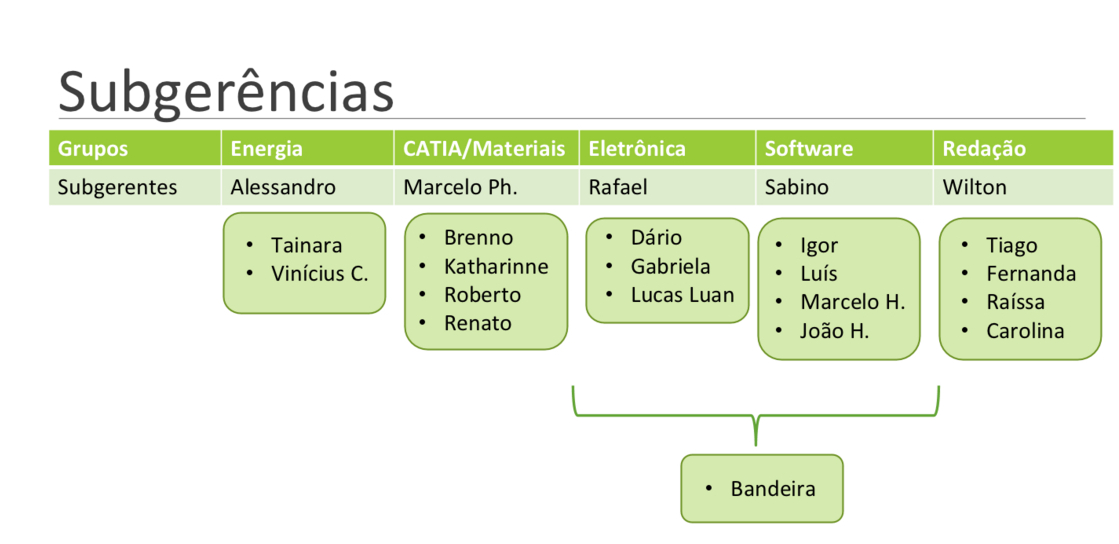
\includegraphics[width=350px, scale=0.5]{figuras/time}
  \caption{Subgerências}
\label{fig:time}
\end{figure}

Como pode ser visto, cada time irá tratar de uma  parte específica do projeto ligado a cada uma das cinco engenharias presentes no Campus FGA. Cada um desses grupos tem atividades próprias que remetem a área de conhecimento e atuação da engenharia que estuda.

O backlog do produto é gerenciado pelos Products Managers e dividido aos Scrum Masters (Subgerente). Cada time de desenvolvimento trabalha a partir de um Sprint Backlog destinado a cada subgerente naquela semana de desenvolvimento e validado no dia da reunião de revisão da sprint.


\section{Cenário de Implementação do CIAC}

\subsection{Locais de Implementação}

Devido a maior incidência de acidentes envolvendo fatalidades, que ocorrem nas rodovias brasileiras simples de mão dupla, em comparação com as cidades, essas foram escolhidas como locais de implementação do sistema.


\subsection{Escolha dos Tipos de Veículos participantes do CIAC}

Em 2013, a PRF registrou um número de 186.474 acidentes nas rodovias federais brasileiras. Em 2014, tínhamos uma frota de 81,3 milhões de veículos.

Os automóveis apresentaram o maior percentual de envolvimento nos acidentes de trânsito nas rodovias e também mortes entre todos os modelos de transporte, em função do maior número da frota circulante. A figura a seguir nos traz números exatos:

\begin{figure}[h!]
  \centering
  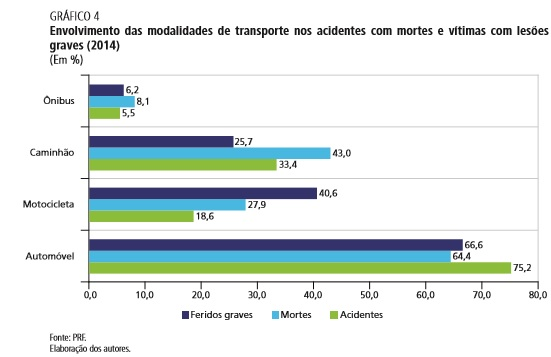
\includegraphics[width=350px, scale=0.5]{figuras/niveisacidente}
  \caption{Envolvimento das Modalidades de Transporte}
\label{fig:time}
\end{figure}

O Sistema será implantado somente em veículos automotores terrestres, com exceção de ciclomotores e motocicletas, devido a alta incidência dos mesmos em acidentes fatais em rodovias brasileiras.
